\documentclass[journal]{IEEEtran}
\usepackage{blindtext}
\usepackage{graphicx}
\usepackage{amsmath}
\usepackage{graphicx}
\usepackage{tabu}
\usepackage{caption} 
\captionsetup[table]{skip=10pt}
\graphicspath{ {images/} }
\DeclareMathOperator*{\argmax}{\arg\!\max}

% correct bad hyphenation here
\hyphenation{op-tical net-works semi-conduc-tor}

\usepackage{hyperref}

\begin{document}
%
% paper title
% can use linebreaks \\ within to get better formatting as desired
\title{Automatic Synthesis of Notes Based on Carnatic Music Raga Characteristics}

\author{Janani~Varadharajan\href{mailto:jananiva@outlook.com}, \and Guruprasad~Sridharan\href{mailto:guruprasad.sridharan@gmail.com}, \and Vignesh~Natarajan\href{mailto:vignesh.natarajan@gmail.com}, \and Rajeswari~Sridhar\href{mailto:raji.sridhar@gmail.com}, \\Department of Computer Science and Engineering
\\College of Engineering, Guindy}

% make the title area
\maketitle

\markboth{Advanced Computing, Networking and Informatics- Volume 1, Volume 27 of the series Smart Innovation, Systems and Technologies pp 145-152}%
{Shell \MakeLowercase{\textit{et al.}}: Bare Demo of IEEEtran.cls for Journals}

\begin{abstract}
%\boldmath
In this paper, we propose two methods to automatically generate notes (Swaras) conforming to the rules of a given Raga in Carnatic music. The proposed methods require training examples for learning the probability model of the chosen Raga and no hand-coded rules are required. Since the methods are purely statistical in nature, it is easy to extend them to work with a large number of Ragas. Each proposed method involves a Learning Phase and Synthesis Phase. In the Learning Phase, an already existing composition of the chosen Raga is used to learn the transition probabilities between Swara sequences based on the Raga lakshana characteristics. In the Synthesis Phase, using the previously constructed transition matrix, Swaras are generated for the desired Raga. We describe two methods - one using First Order Markov Chains and the other based on Hidden Markov Models. Both the methods are validated based on feedback from experts trained in Carnatic music. 
\end{abstract}

\begin{IEEEkeywords}
Carnatic Music, Markov Chain, HMM, Sequence Models.
\end{IEEEkeywords}

\IEEEpeerreviewmaketitle

\section{Introduction}

\subsection{Terminology}
\textbf{Swara} - A Swara is the fundamental unit of Classical Music [1]. A Swara can be analogously understood as a musical note. The basic Swaras in Carnatic music are seven in number and they are as follows: Sa, Ri, Ga, Ma, Pa, Da, Ni.\\

\textbf{Raga} - A Raga is an arrangement of notes in a predefined manner (musical scale) where the position and neighbourhood of each Swara(note) depends on the Raga lakshana of a Raga. The Raga lakshana includes Aarohana (ascending arrangement of notes), Avarohana (descending sequence of notes), the Amsa (characteristic phrase), the frequently used starting note, most frequently used note, ending note, note not used, etc.\\

\textbf{Aarohana} - Aarohana, Arohana, Arohanam or Aroha, in the context of Indian classical music, is the ascending scale of notes in a Raga. The notes ascend in pitch from the lower tonic towards the upper tonic.\\

\textbf{Avarohana} - Avarohana, Avarohanam or Avaroha, in the context of Indian classical music, is the descending scale of any Raga. The notes descend in pitch from the upper tonic down to the lower tonic, possibly in a crooked manner.
In our work, we use the Raga lakshana like Aarohana, Avarohana and Amsa (Characteristic phrase) of each Raga as features to construct a stochastic transition model which is used for synthesis.\\

\textbf{Melakartha} - A collection of fundamental ragas (musical scales) in Carnatic music (South Indian classical music). Melakartha ragas are parent ragas from which other ragas may be generated.

\subsection{Fundamental Idea}
The Ragas are defined not only by the different Swaras that are used to compose it, but also the order of occurrence of these Swaras and one or more characteristic Swara phrases occurring frequently in the composition, thereby giving the Raga an unique signature or an identity. Thus, it is not possible to simply use permutations and combinations of different Swaras to compose a melody in a particular Raga.  For instance, the Ragas \textbf{Shankarabharanam} and \textbf{Kalyani} are both Melakartha Ragas, meaning they have all seven basic Swaras in their \emph{Aarohana} and \emph{Avarohana}.\\

\textbf{Shankarabharanam}:\\ 
Aarohana : $S\ R_2\ G_3\ M_1\ P\ D_2\ N_3\ S$\\   
Avarohana : $S\ N_3\ D_2\ P\ M_1\ G_3\ R_2\ S$\\  

\textbf{Kalyani}:\\
Aarohana: $S\ R_2\ G_3\ M_2\ P\ D_2\ N_3\ S$\\
Avarohana: $S\ N_3\ D_2\ P\ M_2\ G_3\ R_2\ S$\\

If mere permutations and combinations of Swaras are used to generate compositions in these Ragas, one would not be able to easily identify which Raga a particular composition follows, if the compositions do not use the Swara ‘M’. The characteristic phrases must be accentuated well enough in the composition to enable correct identification of the Raga.\\  

In this paper, we describe an algorithm that learns the characteristics of Ragas and synthesizes sequences conforming to the properties of that particular Raga. The primary motive of this paper is to demonstrate the ability of a probabilistic algorithm to understand the characteristics of a Raga and reproduce sequences of the same Raga that do not delve from the rules of the said Raga.\\

This paper is organized as follows: Section 2 talks about the related work in this field, Section 3 explains the proposed method, Section 4 discusses the assumptions and constraints that exist in the method proposed, Section 5 talks about the results and Section 6 concludes the paper with possible future extensions.\\

\section{Related Work}
Sahasrabuddhe in \cite{saha} talks about generating automatic and computer assisted notes that correspond to a particular Raga by constructing a Finite State automata for the Raga, with each states in the Finite State Automata being the alaps (or) phrases of the Raga. The paper claims that remembering the last two notes can produce reasonable performance in a majority of ragas. The authors have further stated that preserving information about elongation, grace notes, and/or successor selection frequencies often enhances the quality of performance.\\

Dipanjan Das et al in \cite{das} investigated the generation of ‘Aarohanas’ and ‘Avarohanas’ present in each Raga that conform to the Hindustani Classical Music for the purpose of discovering and identifying new sequences. This idea implements a Finite State Machine (FSM) which was proposed by \cite{saha} that generates a sequence of Swaras that conforms to the rules of a particular Raga. In \cite{das}, the authors designed a probabilistic finite state machine that generates only the Avarohana and Aarohana of the said Raga. The FSM used in the paper can be looked upon as a bigram model of three most frequent notes along with their probabilities that they follow while moving in either direction so as to generate the ascending and descending sequences of the particular Raga. The FSM for each Raga was constructed manually as the idea deals with only three most frequently occurring notes. Once the FSM created the ascending and descending notes, an algorithm is run on it to generate one instance or sample of the said Raga. This algorithm takes the number of notes and the start note of the Raga as input. Output of the entire process would be a sequence conforming to a particular Raga which was generated upon constructing a sample of the Aarohana and Avarohana of the same. The main drawback that we have identified from this paper is that, a sequence generated using a randomized approach without any defined rules to monitor the occurrence and position of the notes will result in a sequence that does not conform to the characteristics of the Raga.\\

Subramanian in his landmark paper \cite{subra}, talks about generating computer music from skeletal notations, along with the gamakkas that produce a smooth transition from one Swara to another. The proposed system uses user defined gamakkam definition files for each Raga. Addition of gamakkas depend on a) The Raga b) The context in which the note occurs and c) The duration of the note. Gamakkams can be modeled in different ways. One method would be to analyze a large number of recordings sung by music experts and extract common features for each note of the Raga. This requires a system that can identify note boundaries and transcribe live music into notation format.

\section{Method}
The method to generate notes for a Raga is given in Figure 1. The following subsections discuss the proposed methods to generate Raga notes.
\subsection{First Order Markov Chain}
\subsubsection{Learning Phase}
The idea of using Markov chains was inspired by the work of Simone Hill in \cite{hill}. The learning phase involves the computation of the probability with which the Swaras follow one another. Note sequences (transcripts) of existing compositions of the chosen Raga are input to the system in the form of text and the algorithm constructs a 16*16 (seven basic Swaras along with their subtypes) state transition matrix for the Raga based on this sequence. This matrix stores the state transition probability from one Swara to another in a sequence. By this way, frequent bigrams of the chosen Raga are assigned high probabilities.\\

\subsubsection{Synthesis Phase}
In the synthesis phase, a sequence of Swaras pertaining to the desired Raga is generated based on the probabilities in the transition matrix of the Markov Chain. Samples are drawn using a Pseudo Random Number generator based on the cumulative probability for transitions from each input Swara. The initial Swara is chosen based on a starting probability distribution estimated using multiple compositions of the same Raga. As a result of sampling according to Markovian distribtuion, we get a sequence of Swaras of desired length.\\

\subsubsection{Text to Music Phase}
In this phase, each of the sixteen Swaras is assigned a frequency relative to a chosen fundamental frequency based on the rules enforced by the Raga (scale). The composition generated in the previous phase is fed into this phase which then maps the Swaras in the composition to its corresponding frequency and subsequent generation of music is done using Matlab with Karplus-Strong string synthesis algorithm.

\subsection{Hidden Markov Model}
Hidden Markov Models (HMMs) are used to model finite discrete or continuous observation sequences when the state transitions cannot be observed directly \cite{stein}. HMMs have been employed successfully for speech recognition, speech synthesis, machine translation, parts-of-speech tagging, cryptanalysis, gene prediction, etc. HMM is an extension to the finite state Markov model which makes it more applicable to real-world processes, where the sequence of states cannot be observed. HMMs have been used for generation of chord harmonizations in Western Music \cite{hill}. The ability of HHMs to capture complex harmonies from the training sequence makes it attractive for generation of melodies. We propose to use HMM for generation of Carnatic music and provide a comparison of its performance against the method previously discussed, in the Results and Analysis section.

\subsubsection{Algorithm}
The algorithm takes as input a Raga chosen by the user and a training sequence. The training sequence consists of Swaras which constitute a musical piece conforming to the chosen Raga. The algorithm learns from the training sequence and outputs a sequence of generated Swaras conforming to the chosen Raga.\\

\begin{figure}[h]
\caption{Block Diagram of the notes synthesis system}
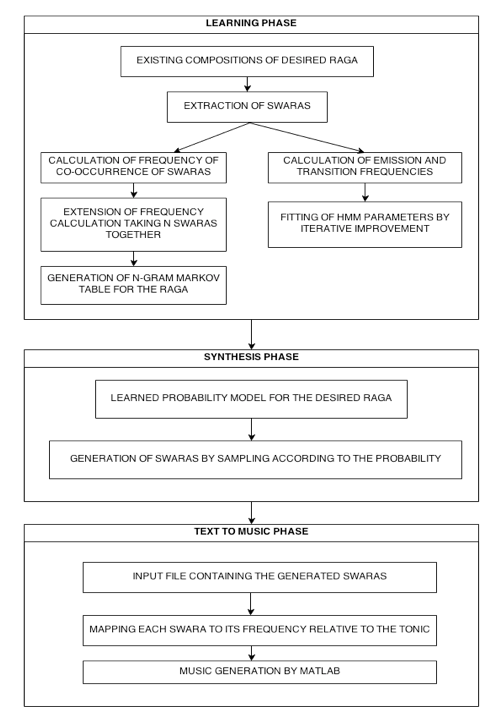
\includegraphics{flowchart}
\end{figure}

The Hidden Markov Model is composed of three probability distributions namely Transition, Emission and Initial probability distributions. The parameters include number of hidden states and visible states, and the vocabulary used(set of symbols emitted).\\

We use a finite discrete HMM model for generating the sequence of Swaras. The hidden states correspond to the characteristic phrases (a group of Swaras). The emitted symbols correspond to the Swaras.\\

The intuition behind using HMMs is that they are better at capturing this phrasal structure of Swaras from the training examples which is necessary for generating complex and more nuanced harmonies.\\

HMMs are typically described using a three-tuple representation \cite{hill} $M = (A, B, \Pi)$, where\\
$A$ - $N \times N$ matrix which describes transition probability between states.\\
$B$ - Emission probability distribution ($B = {b_1, b_2, \hdots , b_N}$).\\
$Π$ - Initial probability distribution over states.\\
$N$ - Number of hidden and visible states.\\
$a_{ij}$ - Transition probability between $i^{th}$ state and $j^{th}$ state.\\
$b_i$ - Emission probability for the $i^{th}$ state.\\
$X_t$ - Random variable which denotes the state of the system at time $t$.\\
$Y_t$ - Random variable which denotes the symbol emitted at time $t$.\\

The aim of the learning phase is to find a model $M$̂ in the model space $M^*$ such that

\begin{align*}
    M = \argmax_{M \epsilon M^*} P(Y|M) 
\end{align*}

\emph{Baum-Welch algorithm}, a specialization of \emph{Expectation-Maximization algorithm} is used for learning the model. It learns that model which maximizes the likelihood of observing the sequence training sequence Y.

Number of hidden states were chosen by a cross-validated approach. Scikit-learn package for Python provides an implementation for categorical HMM \cite{scikit}\cite{scipy} which was used for the implementation and evaluation.\\

\textbf{Steps:}
\begin{enumerate}
\item Fetch the training sequences for the chosen Raga from the database.
\item Start with some random initialization values for the 3-tuple.
\item Apply forward and backward passes of the Baum-Welch algorithm on all the training sequences to update the conditional model variables for achieving Expectation-Maximization and repeat until convergence based on threshold $T$.
\item Repeat the algorithm multiple times with different initialization values and find the model with the best score.
\item Sample from the trained HMM model to henerate output sequence of desired length with starting symbol (\emph{Swara}) chosen by sampling from initial distribution derived from training sequences\\
\end{enumerate}

\section{Limitations}
\begin{itemize}
  \item The proposed system does not handle the gamakkas of the generated composition. 
  \item The system doesn't try to fit tala (time singature) to the generated composition.
  \item The system proposed is purely statistical in nature so the quality of the generated composition is limited by the richness of corpus data used in the learning phase.
\end{itemize}

\section{Results and Analysis}
The aim of the experiment was to measure the goodness of the notes generated by the generative model and to validate whether the notes correspond to the Raga given as input.\\
Six people trained in Carnatic music took part in the experiment. A dataset consisting of songs in .wav format was prepared. The participants were asked to rate each musical composition in the dataset on a scale of 1 to 5, based on their perceived similarity to the corresponding Raga to which the composition originally belonged.\\

\begin{table}[ht]
\centering
\caption{Table showing the mean and standard deviation (enclosed by parantheses) of scores on each Raga for both the methods}
\begin{tabu} to 0.5\textwidth { | X[l] | X[c] | X[r] | }
 \hline
 Raga & Hidden~Markov~Model & First Order Markov Chain \\
 \hline
 Thodi & 1.75 (0.41) & 1.5 (0.45) \\
 \hline
 Shankarabharanam & 2.5 (0.63) & 2.5 (0.63) \\
 \hline
 Mohanam & 3 (0.45) & 2.75 (0.69) \\
 \hline
 Malahari & 2.25 (0.52) & 1.75 (0.69) \\
 \hline
 Kalyani & 2.5 (0.71) & 2.5 (0.55) \\
 \hline
\end{tabu}
\label{table:1}
\end{table}

\section{Conclusion}
In this paper, we have compared the performance of First Order Markov Model with that of HMM for synthesis of Carnatic Music. The result indicates that even though HMM performs better than Bigram model, the performance is poor on an absolute scale. Future work can focus on the evaluating the use of discriminative models such as Conditional Random Fields for this problem. It is also worthwhile to explore the use of sequence statistics to construct a scoring function for automated scoring of the generated compositions.

% use section* for acknowledgement
\section*{Acknowledgment}
The authors would like to thank the Center for Technology Development and Transfer, College of Engineering, Guindy, Anna University for funding this project.

% Can use something like this to put references on a page
% by themselves when using endfloat and the captionsoff option.
\ifCLASSOPTIONcaptionsoff
  \newpage
\fi

% trigger a \newpage just before the given reference
% number - used to balance the columns on the last page
% adjust value as needed - may need to be readjusted if
% the document is modified later
%\IEEEtriggeratref{8}
% The "triggered" command can be changed if desired:
%\IEEEtriggercmd{\enlargethispage{-5in}}

% references section

% can use a bibliography generated by BibTeX as a .bbl file
% BibTeX documentation can be easily obtained at:
% http://www.ctan.org/tex-archive/biblio/bibtex/contrib/doc/
% The IEEEtran BibTeX style support page is at:
% http://www.michaelshell.org/tex/ieeetran/bibtex/
%\bibliographystyle{IEEEtran}
% argument is your BibTeX string definitions and bibliography database(s)
%\bibliography{IEEEabrv,../bib/paper}
%
% <OR> manually copy in the resultant .bbl file
% set second argument of \begin to the number of references
% (used to reserve space for the reference number labels box)
\begin{thebibliography}{1}

\bibitem{kopka}
H.~Kopka and P.~W. Daly, \emph{A Guide to \LaTeX}, 3rd~ed.\hskip 1em plus
  0.5em minus 0.4em\relax Harlow, England: Addison-Wesley, 1999.
\bibitem{pichu}
Sambamoorthy, Pichu. South Indian Music.~Vol.~4.~Indian Music Publishing House, 1969.
\bibitem{saha}
H.~V. Sahasrabuddhe, \emph{Analysis and Synthesis of Hindustani Classical Music}, University of Poona, 1992.
\bibitem{das}
Das, Dipanjan, and Monojit Choudhury. \emph{Finite state models for generation of Hindustani classical music}. Proceedings of International Symposium on Frontiers of Research in Speech and Music, 2005.
\bibitem{subra}
M.~Subramanian, \emph{Generating Computer Music from Skeletal Notations for Carnatic Music Compositions}, Proceedings of the 2nd CompMusic Workshop, Istanbul, Turkey, July 2012.
\bibitem{hill}
Simone Hill, Markov Melody Generator, 2011.
\bibitem{stein}
D.~Steinsaltz, and D.~Wessel. In Progress, \emph{The Markov Melody Engine: Generating Random Melodies With Two-Step Markov Chains}. Technical report, Department of Statistics, University of California at Berkeley. 
\bibitem{kohl}
C.~ Kohlschein. \emph{An introduction to hidden Markov models}. Probability and randomization in computer science, seminar in winter semester, Aachen University, 2006/2007. 
\bibitem{scikit}
Pedregosa, Fabian, et al. \emph{Scikit-learn: Machine learning in Python}. The Journal of Machine Learning Research 12 (2011): 2825-2830. 
\bibitem{scipy}
Oliphant, Travis E. \emph{Python for scientific computing}. Computing in Science \& Engineering 9.3 (2007): 10-20.
\end{thebibliography}

\end{document}


